\subsection{Ray tracing simulations}

\textbf{You will:}

\begin{itemize}
    \item Define a geometrical source with Gaussian profiles.
    \item Define screens and slits.
    \item Observe the changes in phase space when the beam propagates.
    \item Study the effect of a slit or aperture.
\end{itemize}

\textbf{Questions:}

\textbf{i)} Create a geometric source with Gaussian profiles  (in real space: 1 mm $\times$ 0.1 mm, in divergence space: 1 mrad $\times$ 0.1 mrad; rms values, H $\times$ V) and add several screens at 0 (source position), 0.5, 0.75 and 1 m from the source. See the tilt of the (x,x’) (horizontal) and (z,z’) (vertical) diagrams. 

\textbf{ii)} Define an aperture (500 $\times$ 50 $\mu$m) in the first screen and see its effect in the other screens placed downstream from the beam. 


\textbf{Answer}

\begin{figure}[H]
\label{fig:bp-fig1}
\caption{Evolution of the phase space. Top:  in X (horizontal), bottom: in Z (vertical).}
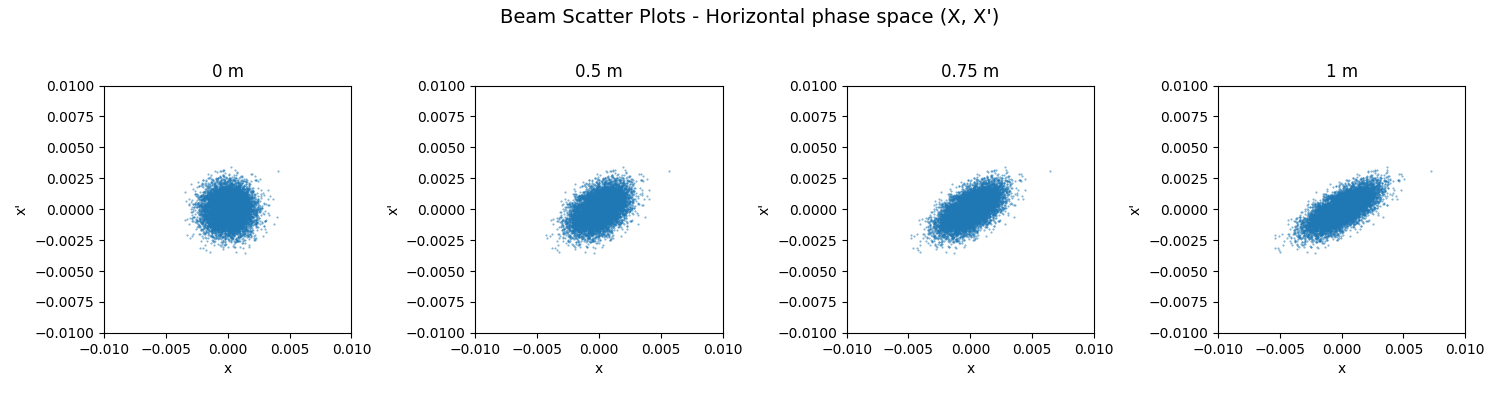
\includegraphics[width=0.9\textwidth]{beam-propagation/fig1a.png}
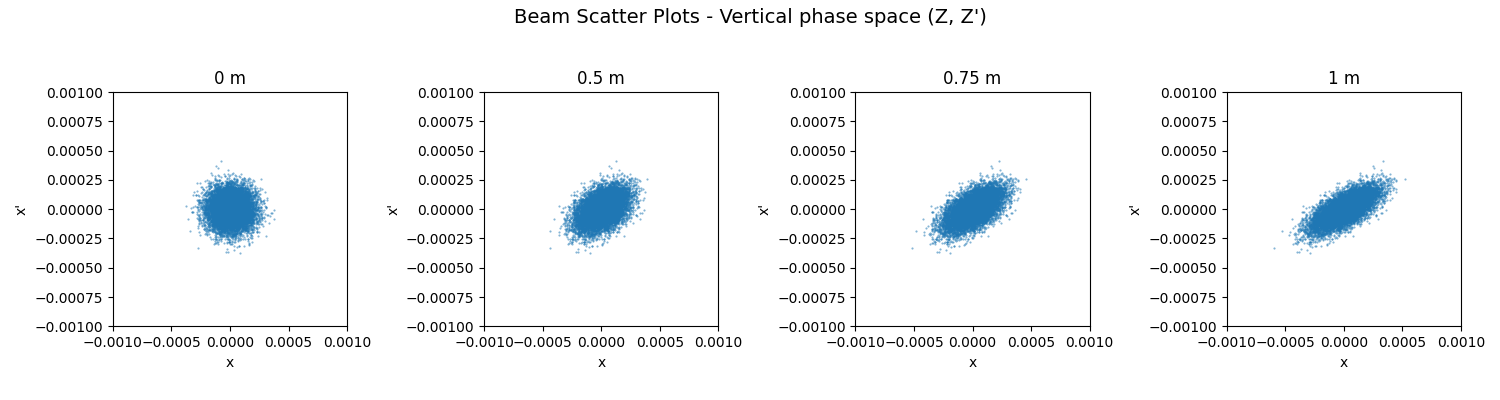
\includegraphics[width=0.9\textwidth]{beam-propagation/fig1b.png}
\end{figure}

\begin{figure}[H]
\label{fig:bp-fig2}
\caption{Evolution of the phase space. Effect of a slit in the first screen. Top:  in X (horizontal), bottom: in Z (vertical).}
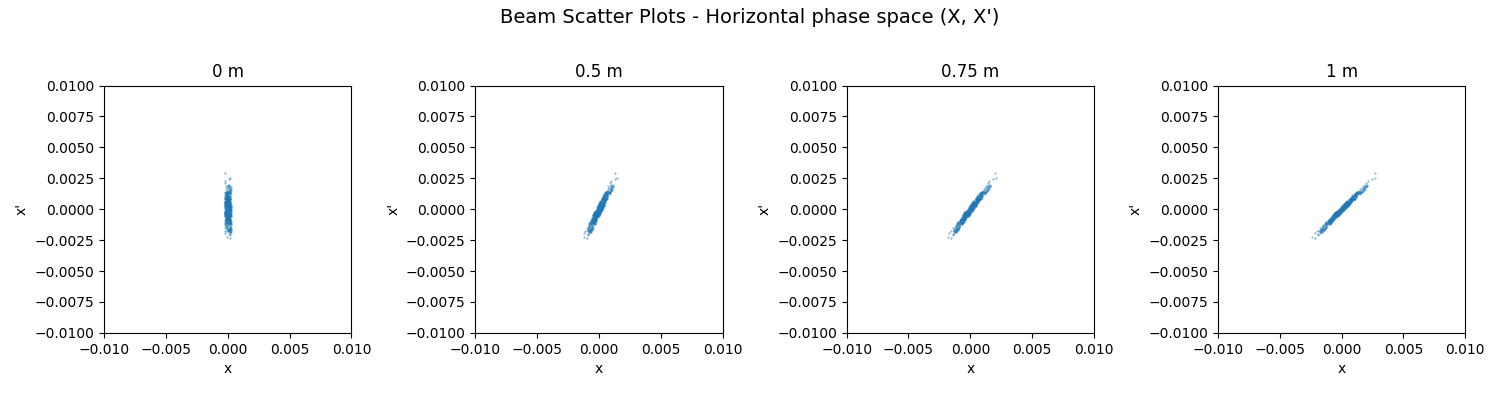
\includegraphics[width=0.9\textwidth]{beam-propagation/fig2a.png}
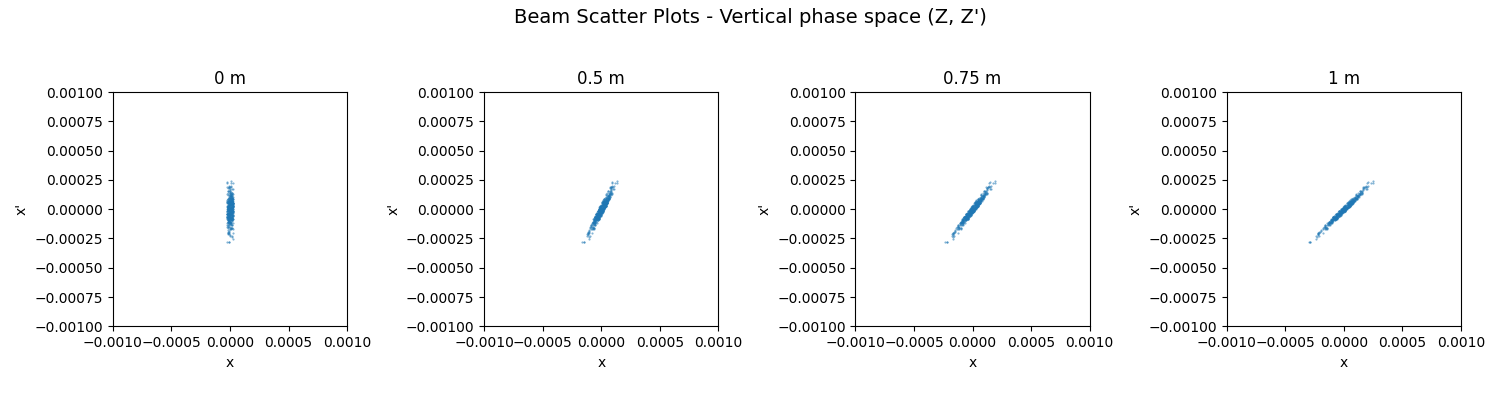
\includegraphics[width=0.9\textwidth]{beam-propagation/fig2b.png}
\end{figure}

Note that instead of defining the different screens, one can directly plug a “Plot XY”  to the source and widget and use “Position of the image” = Retraced and play with the distances. 



